% DNS defined in the intro!
\subsection{Incompressible DNS Application}
\label{sec:dns_full}

In many fluid dynamics applications, turbulence plays a
dominant role. Unfortunately, turbulence is 
notoriously complex and difficult to model. Even though the governing equation, Navier-Stokes equation, for the turbulent flow is well-defined, the understanding of turbulent flow is still a challenging problem. One of the reason why it is difficult to study is that the length and time-scale of turbulent flow becomes smaller as Reynolds number $Re$ increases. ($Re$ the ratio of inertia force to viscous force of flow.) In Direct numerical simulation (DNS) one allocates grids as many as necessary, and the necessary grids size increases as $Re$ increases. As far as we know the largest wall-bounded DNS is performed by (Lee \& Moser 2015, JFM) and 240 billions degree of freedom has been used for the flow between parallel planes at $Re = 250000$. However, higher $Re$ simulation with larger problem size is required to answer many unsolved problems in fluid dynamics. Hence, it is natural to prepare the simulation code for next generation computers.

Poongback, the DNS code for incompressible channel flow, has already shown excellent performance and has been already used in several researchers. Especially, it has been used for the simulation by (Lee \& Moser 2015, JFM) and generating the data for virtual flow laboratory in Johns Hopkins Turbulence Data Base (Cite here). The spectral-Galerkin method and B-spline collocation method are used in PoongBack. There are four main parts in Poongback, data transpose with 2D decomposition, multiple 1D FFTs, solving linear equations with real matrix and complex vectors and I/O in HDF5 format. For I/O, we uses customized I/O library, ESIO, but we have not tested its performance for this work. The data transpose 2D decomposition and multiple 1D FFTs are done by FFTW3.3 library. Note that FFTW3.3 (and above) library support the use of MPI but it is implemented for 1D data decomposition. To overcom this issue, we created two MPI-subcommunicators, and called FFTW for data transpose and FFTs seperately. Also, we have implemented customized banded-matrix solver to linear equations. See (Lee, Malaya, Moser 2013, SC) for more detail about PoongBack.

\begin{figure}[htb]
 \begin{center}
   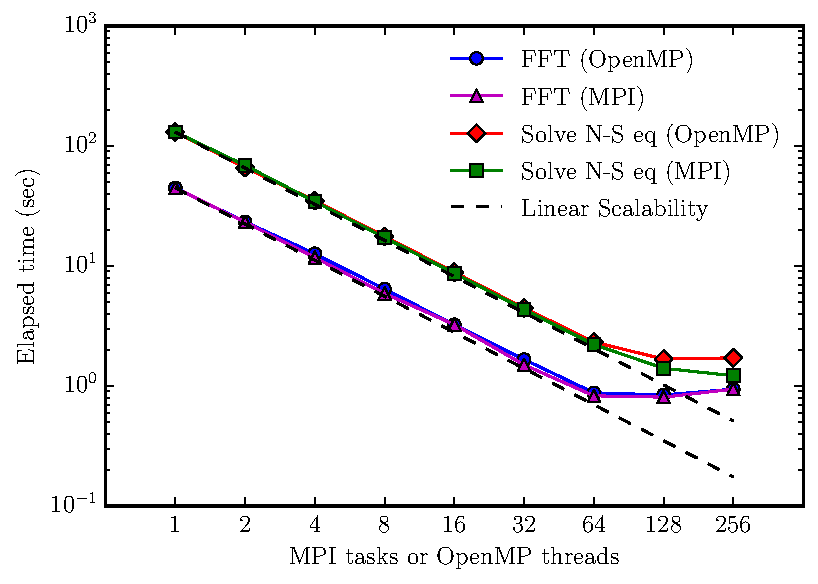
\includegraphics[width=0.45\textwidth]{DNS_FFT_Wave}
   \caption{Strong scaling result of 1D FFTs and Solving N-S equations in wavespeace for single timestep.}
   \label{fig:DNS_strong_scale_fft_wave}
 \end{center}
\end{figure}

For this study the grid size is used $1024\times128\times512$ and the grid size is comparable for $Re_\tau = 180$ simulation by (cite here). Throughout the every benchmark cases, the MCDRAM is used as a cache memory between processors and DRAM. Figure~\ref{fig:DNS_strong_scale_fft_wave} shows the strong scaling performance of 1D FFTs (real-to-complex, complex-to-real and complex-to-complex) and floating point operations with complex numbers including linear equation solvers. The linear equation, $A\mathbf{x} = \mathbf{b}$, is solved to compute B-spline coefficients. $A$ is a diagonal dominant banded matrix with additional non-zero elements in several top and bottom rows. $\mathbf{x}$ and $\mathbf{b}$ is complex vectors. As shown in the Figure~\ref{fig:DNS_strong_scale_fft_wave}, FFTs and floating point operations shows good scalability in both OpenMP only and MPI only cases with upto 64 processors. Using MPI only shows slightly better performance but the difference is negligible. After the hyperthread\todo{it this right term?} is used performance with FFTs are decreased because FFTs are bounded by the memory access not by floating point operations. On the otherhands, the kernel with linear equation shows slight performance increases even with the hyperthreads. Interestingly, using MPI shows better performance than OpenMP. This maybe due to the difference of memory access pattern between two parallelism. \todo{Chris, is this make sense?}.


\begin{figure}[htb]
 \begin{center}
   \includegraphics[width=0.45\textwidth]{DNS_Transpose}
   \caption{Strong scaling result of data reorder and MPI communication; OpenMP is not used.}
   \label{fig:DNS_strong_scale_transpose}
 \end{center}
\end{figure}

\begin{figure}[htb]
 \begin{center}
   \includegraphics[width=0.45\textwidth]{DNS_Parallelism}
   \caption{Comparison of MPI$\times$OpenMP configuration}
   \label{fig:DNS_MPI_OpenMP}
 \end{center}
\end{figure}

\begin{figure}[htb]
 \begin{center}
   \includegraphics[width=0.45\textwidth]{DNS_full_timestep}
   \caption{Strong scaling result of total elapsed time for single timestep; (MPI tasks $\times$ OpenMP threads) is hybrid configuratation which showed  the best performance.}
   \label{fig:DNS_strong_scale_total_elapsed_time}
 \end{center}
\end{figure}





\todo{if we merge this with the previous section, we can have an intro
to dns and then talk about each in detail}

